\section{Prior for DUMs Details}
\label{subsec:appendix_prior}

For all the prior experiments we use the default training settings in \cref{subsec:appendix_training} and \cref{tab:appendix_default_hyper}. In the following experiments, we vary the \textit{entropy regularization} $\lambda$ and the \textit{evidence prior} $n^{prior}$ for NatPN, and the choice of kernel for DUE. 

Before starting the training, we inject the artificial aleatoric noise by reassigning the target $y$ with a randomly chosen class. Two datasets with different degree of noise are used, where 10\% and 20\% of all the labels in the training dataset are reassigned.  

\begin{figure}[!htb]
    \centering
    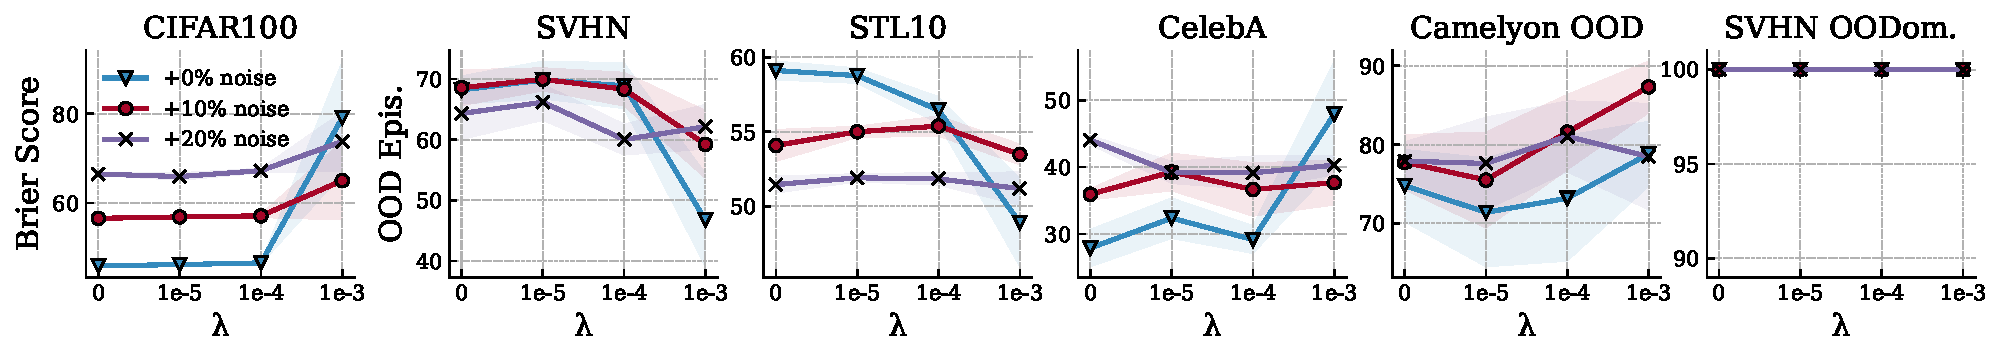
\includegraphics[width=\textwidth]{sections/008_iclr2023/figures/prior_entropy_brier_epis.pdf}
    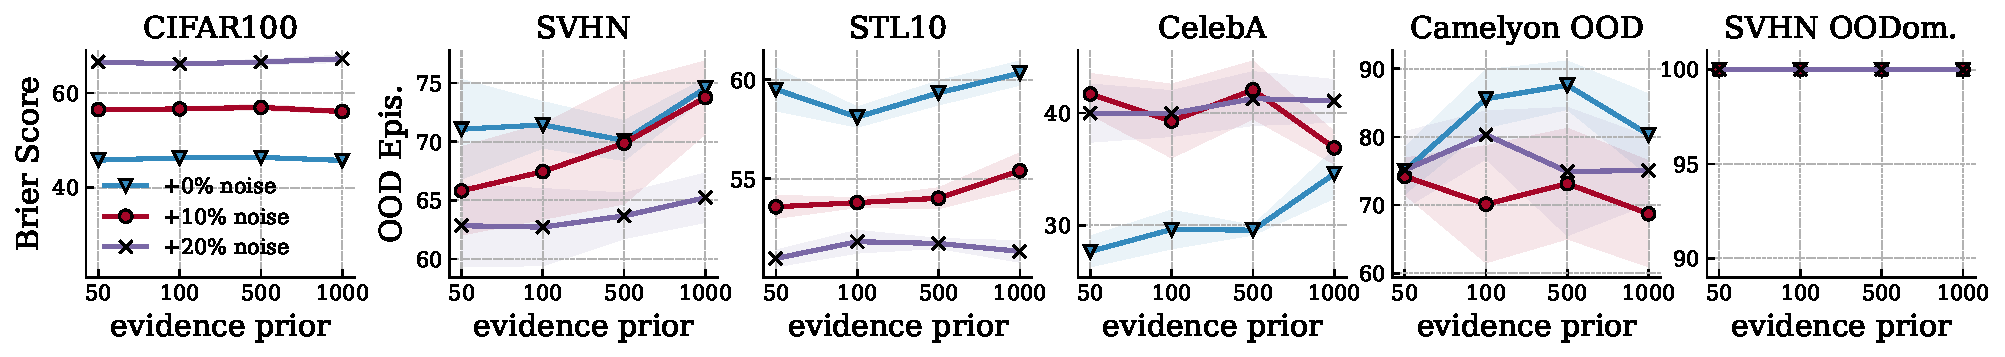
\includegraphics[width=\textwidth]{sections/008_iclr2023/figures/prior_pseudo_brier_epis.pdf}
    
    \caption{Results of enforcing different \textbf{prior} in NatPN on CIFAR100 by changing the (top) \textit{entropy regularization} $\lambda$ and the (bottom) \textit{evidence prior} $n^{prior}$. Different priors do not lead consistent results improvements.}
    \label{fig:prior_ood_brier}
\end{figure}